\documentclass[11pt]{article}
\usepackage[margin=0.85in]{geometry}
\usepackage{amsmath,amssymb,amsthm}
\usepackage{graphicx}
\usepackage{microtype}
\usepackage{xcolor}
\usepackage{hyperref}
\hypersetup{colorlinks=true,linkcolor=blue!55!black,urlcolor=blue!55!black,citecolor=blue!55!black}
\newtheorem{theorem}{Theorem}
\newtheorem{lemma}{Lemma}
\newcommand{\Tr}{\operatorname{Tr}}
\newcommand{\id}{\operatorname{id}}
\newcommand{\cE}{\mathcal E}
\newcommand{\cL}{\mathcal L}
\newcommand{\cP}{\mathcal P}
\newcommand{\cB}{\mathcal B}
\newcommand{\GammaS}{\Gamma_\sigma}
\title{Strict $p$-Dirichlet positivity for Poisson-type quantum generators\\a partial answer to arXiv:2207.06422}
\author{Candidate partial-result packet}
\date{11 August 2026}

\begin{document}
\maketitle

\begin{center}
\fbox{\parbox{0.91\linewidth}{\textbf{Status:} candidate partial result likely valid. The open strict-positivity assertion is proved for primitive Poisson-type generators and positive sums of them. This includes the paper's explicit primitive $[\sigma]_{p,0}$-DBC example that is not GNS detailed balanced. The general infinitesimal problem remains open.}}
\end{center}

\section{Source question}

Li and Lu ask whether, for $1<p<2$, every primitive Lindbladian $\cL$
satisfying $[\sigma]_{p,0}$ detailed balance obeys
\begin{equation}\label{eq:source-question}
 \cE_{p,\cL}(\GammaS^{-1}(\rho))>0
 \qquad(\rho>0,\ \rho\ne\sigma).
\end{equation}
They prove this under GNS detailed balance, and for $p=2$ under the weaker
$[\sigma]_{2,0}$ condition, but leave the general case open~\cite{LiLu}.

\begin{center}

\includegraphics[width=0.98\textwidth]{figures/open_problem_crop.png}

\smallskip
\emph{The exact open question on page 42 of the source.}
\end{center}

The same paper supplies an especially useful test case.  For
$0<\eta<1/2$, let
\[
 K_1=\begin{pmatrix}\sqrt\eta&0\\0&\sqrt{1-\eta}\end{pmatrix},
 \qquad
 K_2=\begin{pmatrix}0&\sqrt\eta\\\sqrt{1-\eta}&0\end{pmatrix},
\]
and $\Phi(X)=K_1^*XK_1+K_2^*XK_2$.  Its invariant state is
$\sigma=\operatorname{diag}(\eta,1-\eta)$, and $\Phi-\id$ is primitive and
$[\sigma]_{p,0}$ detailed balanced, but not GNS detailed balanced.

\begin{center}
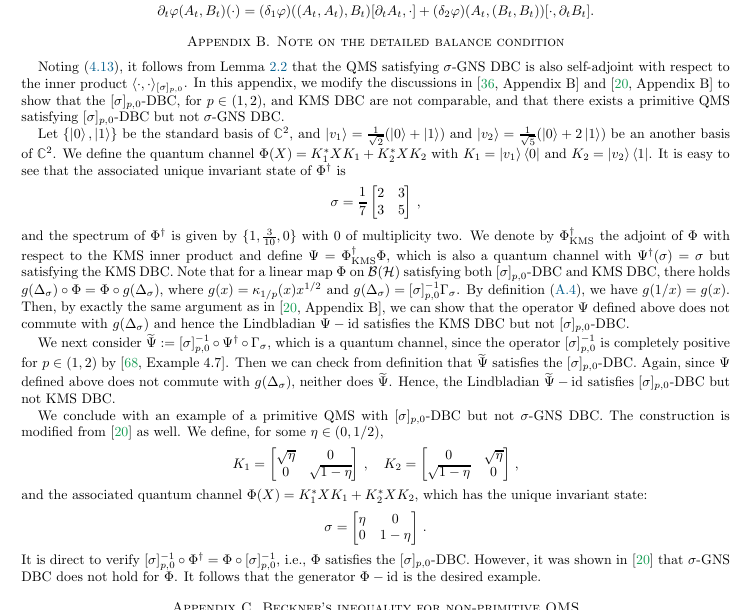
\includegraphics[width=0.98\textwidth]{figures/appendix_example_crop.png}

\smallskip
\emph{The source's non-GNS primitive example, page 44.}
\end{center}

\section{The partial theorem}

For $1<p<\infty$ and $q=p/(p-1)$, write
\[
 \|X\|_{p,\sigma}
 =\left(\Tr\left|\GammaS^{1/p}(X)\right|^p\right)^{1/p},
 \qquad
 I_{q,p}(X)=\GammaS^{-1/q}
 \left(\GammaS^{1/p}(X)^{p-1}\right)
\]
for $X>0$.  The source's normalization is
\[
 \cE_{p,\cL}(X)
 =-\frac{pq}{4}\langle I_{q,p}(X),\cL X\rangle_{\sigma,1/2},
 \quad
 \langle A,B\rangle_{\sigma,1/2}
 =\Tr(\sigma^{1/2}A^*\sigma^{1/2}B).
\]

\begin{theorem}[Poisson-type strict positivity]\label{thm:main}
Let $\Phi_1,\ldots,\Phi_m:\cB(\mathcal H)\to\cB(\mathcal H)$ be unital
completely positive maps satisfying $\Phi_k^\dagger(\sigma)=\sigma$, let
$\gamma_k>0$, and set
\[
 \cL=\sum_{k=1}^m\gamma_k(\Phi_k-\id).
\]
Then $\cE_{p,\cL}(X)\ge0$ for every $X>0$ and every $1<p<\infty$.
Equality holds precisely when $\Phi_k(X)=X$ for every $k$.  Consequently, if
$\cL$ is primitive, then
\[
 \cE_{p,\cL}(\GammaS^{-1}(\rho))>0
 \quad\text{for every full-rank state }\rho\ne\sigma.
\]
No detailed-balance assumption is needed for this conclusion.
\end{theorem}

\begin{proof}
First consider one map $\Phi$.  It is a contraction on every weighted
$L_p(\sigma)$ space:
\begin{equation}\label{eq:contract}
 \|\Phi X\|_{p,\sigma}\le \|X\|_{p,\sigma}.
\end{equation}
For completeness, at $p=\infty$ this is the usual operator-norm contraction
of a unital positive map.  At $p=1$, the conjugated map
\[
 \widehat\Phi=\GammaS\circ\Phi\circ\GammaS^{-1}
\]
is completely positive and trace preserving: using
$\Phi^\dagger(\sigma)=\sigma$ gives
$\Tr\widehat\Phi(A)=\Tr A$.  Hence it contracts the trace norm.  Complex
interpolation between these two endpoint spaces gives~\eqref{eq:contract};
the interpolated norm is exactly
$\|X\|_{p,\sigma}=\|\GammaS^{1/p}X\|_p$.

Put $Y=\GammaS^{1/p}(X)>0$.  The weighted duality pairing satisfies
\begin{align*}
 \langle I_{q,p}(X),X\rangle_{\sigma,1/2}
 &=\Tr Y^p=\|X\|_{p,\sigma}^p,\\
 \langle I_{q,p}(X),\Phi X\rangle_{\sigma,1/2}
 &=\Tr\!\left(Y^{p-1}\GammaS^{1/p}(\Phi X)\right).
\end{align*}
Schatten H\"older and~\eqref{eq:contract} therefore yield
\begin{align}\label{eq:holder-chain}
 \langle I_{q,p}(X),\Phi X\rangle_{\sigma,1/2}
 &\le \|Y^{p-1}\|_q\,\|\GammaS^{1/p}(\Phi X)\|_p\\
 &\le \|X\|_{p,\sigma}^{p-1}\|X\|_{p,\sigma}
 =\langle I_{q,p}(X),X\rangle_{\sigma,1/2}.\notag
\end{align}
Thus $\cE_{p,\Phi-\id}(X)\ge0$.

If equality holds, equality holds in the first line of
\eqref{eq:holder-chain}.  Since $1<p<\infty$ and both matrices are positive,
the equality case of Schatten H\"older gives
$\GammaS^{1/p}(\Phi X)=cY$ for some $c\ge0$.  Equality with the leftmost
quantity in~\eqref{eq:holder-chain} forces $c=1$, hence $\Phi X=X$.
The converse is immediate.

The Dirichlet form is linear in the generator, so
\[
 \cE_{p,\cL}(X)=\sum_{k=1}^m\gamma_k
 \cE_{p,\Phi_k-\id}(X).
\]
Every summand is nonnegative, and their sum vanishes exactly at their common
fixed points.  If $\cL$ is primitive, its fixed-point algebra is
$\mathbb C I$, so equality forces $X=cI$.  Finally, when
$X=\GammaS^{-1}(\rho)$ and $\Tr\rho=1$, the normalization gives $c=1$ and
$\rho=\sigma$.
\end{proof}

\section{Application to the paper's missing example}

The explicit Appendix B channel displayed above is unital, fixes $\sigma$ in
the dual, and $\Phi-\id$ is primitive.  Theorem~\ref{thm:main} therefore gives
\eqref{eq:source-question} for this $[\sigma]_{p,0}$-DBC but non-GNS family,
for every $0<\eta<1/2$ and every $1<p<\infty$.  Thus the paper's example
showing that the two detailed-balance classes differ does not create an
exception to strict positivity.

The same argument applies to any generator that can be uniformized, meaning
$\id+\varepsilon\cL$ is a unital completely positive map for some
$\varepsilon>0$: then
$\cL=\varepsilon^{-1}((\id+\varepsilon\cL)-\id)$.

\section{Upgrade attempts and the remaining obstruction}

The strongest extension route was tested rather than silently assumed.

\begin{enumerate}
\item The two non-GNS qubit constructions in Appendix B were implemented
directly.  Differential evolution over the full-rank Bloch ball, at 35
parameter choices, found the unique zero at the invariant state, up to
$2\times10^{-15}$ floating-point error.
\item A general qubit GKSL generator was parametrized by a Hermitian positive
$3\times3$ Kossakowski matrix and a traceless Hamiltonian.  Imposing
$[\sigma]_{p,0}$-DBC gives a six-dimensional real cone.  For 20 sampled
primitive generators at $(\eta,p)=(0.2,1.5)$, global minimization again found
only the invariant-state zero, at residuals below $8\times10^{-17}$.
\item Uniformization does not cover that whole cone.  The primitive
$[\sigma]_{p,0}$-DBC boundary generator with Kossakowski matrix
\[
 C=\begin{pmatrix}1/2&-0.3i&0\\0.3i&1/2&0\\0&0&0\end{pmatrix}
 \quad(\sigma=\operatorname{diag}(0.2,0.8),\ p=3/2)
\]
has spectrum $\{0,-1,-1/2,-1/2\}$, but the Choi matrix of
$\id+\varepsilon\cL$ has a negative eigenvalue for every tested
$\varepsilon>0$, asymptotic to $-0.045\varepsilon^2$.  Hence the proof above
cannot be extended to all generators by taking one Euler step.
\item Passing instead to the genuine channel $e^{t\cL}$ proves positivity of
the finite difference
$\langle I_{q,p}(X),(I-e^{t\cL})X\rangle$, but after division by $t$ and
$t\downarrow0$ strictness may be lost.  A contraction can touch a smooth norm
sphere to first order while entering it at second order.  This is the exact
infinitesimal equality obstruction left by the argument.
\end{enumerate}

The computations are reproducible from the two scripts in \texttt{code/}.
They are evidence and obstruction checks; they are not used in the proof of
Theorem~\ref{thm:main}.

\section{Bounded novelty check and conclusion}

A bounded search through 11 August 2026 covered the run indexes, the exact
open sentence, the paper title and arXiv identifier with the relevant
detailed-balance and Dirichlet-form phrases, and the four later works indexed
as citing the published article.  None claimed this strict-positivity result
or a resolution of the general question.  Novelty confidence is moderate:
the proof uses standard weighted $L_p$ contractivity and may be known as
folklore, but its application to the source's non-GNS example does not appear
to have been recorded.

The general question remains open, but Theorem~\ref{thm:main} removes a broad
and natural class, including the paper's own separating example, and isolates
why the same two-line argument does not automatically cover every
Lindbladian.

\begin{thebibliography}{9}
\bibitem{LiLu}
B. Li and J. Lu,
\emph{Interpolation between modified logarithmic Sobolev and Poincar\'e
inequalities for quantum Markovian dynamics},
J. Stat. Phys. 190 (2023), 161; arXiv:2207.06422.
\url{https://arxiv.org/abs/2207.06422}.

\bibitem{Beigi}
S. Beigi, N. Datta, and C. Rouz\'e,
\emph{Quantum reverse hypercontractivity: its tensorization and application
to strong converses},
Commun. Math. Phys. 376 (2020), 753--794; arXiv:1804.10100.
\url{https://arxiv.org/abs/1804.10100}.
\end{thebibliography}

\end{document}
